If $\vec P$ be a point on the line and $\vec n$ is the normal vector, the equation of the line can be expressed as 
\begin{align}
    & \vec n^T\brak{\vec x - \vec P}=0\\
    & \label{eq:solutions/4/2/2/eq2}\implies \vec n^T \vec x = c
\end{align}
where
\begin{align}
    c= \vec n^T \vec P
\end{align}
From \brak{\ref{eq:solutions/4/2/2/eq1}} and \brak{\ref{eq:solutions/4/2/2/eq2}}, 
\begin{align}
     \vec n^T = \myvec{3 & 2}
\end{align}
We know,
\begin{align}
    &\vec m^T \vec n = 0\\
    &\implies \vec m^T \myvec{3 \\2} = 0\\
    &\implies \vec m ^T = \myvec{-2 & 3}
\end{align}

Now,
\begin{align}
    &\vec n^T \vec P = c \\
    &\implies \myvec{3 & 2} \vec P= 12
\end{align}

$\vec P$ can be
\begin{align}
    \myvec{4\\0}, \myvec{2\\3}, \myvec{0\\6}
\end{align}
Let us take 
\begin{align}
    \vec P =\myvec{2\\3}=\vec q
\end{align}
The circle equation:
\begin{align}
    \vec x^T \vec x + 2 \vec u^T\vec x +f=0
\end{align}
From \brak{\ref{eq:solutions/4/2/2/eq:circle}},
\begin{align}
    &\vec u=\myvec{0\\0}\\
    & f=-13
\end{align}
The points of intersection of the line
\begin{align}
    L: \vec x = \vec q + \mu \vec m \quad ,\mu \in \mathbb R
\end{align}
with the conic section
\begin{align}
    \vec x^T \vec V \vec x +2\vec u^T \vec x+ f=0
\end{align}
are given by 
\begin{align}
    \label{eq:solutions/4/2/2/points of intersection}\vec x_i = \vec q + \mu _i \vec m
\end{align}
where,

\begin{multline}
\mu_i = \frac{1}
{
\vec{m}^T\vec{V}\vec{m}
}
\lbrak{-\vec{m}^T\brak{\vec{V}\vec{q}+\vec{u}}}
\\
\pm
{\small
\rbrak{\sqrt{
\sbrak{
\vec{m}^T\brak{\vec{V}\vec{q}+\vec{u}}
}^2
-
\brak
{
\vec{q}^T\vec{V}\vec{q} + 2\vec{u}^T\vec{q} +f
}
\brak{\vec{m}^T\vec{V}\vec{m}}
}
}
}
\end{multline}
For circle,
\begin{align}
    &\vec V = \vec I\\ 
    & \therefore \mu_i = \frac{1}{13}\lbrak{-5 \pm \rbrak{\sqrt{25- \brak{13-13}13}
    }
    }\\
    & = \frac{1}{13}\brak{-5 \pm 5}\\
    & = 0, -\frac{10}{13}
\end{align}
Using \brak{\ref{eq:solutions/4/2/2/points of intersection}}, the points of intersection are given by
\begin{align}
    \vec x = \myvec{2\\3} , \myvec{\frac{46}{13}\\ \frac{9}{13}}
\end{align}
Points of contact are given by
\begin{align}
    \vec q = \vec V^{-1} \brak{\kappa \vec n - \vec u}\\
    \kappa = \pm \sqrt{\frac{\vec u^T \vec V^{-1} \vec u -f}{\vec n^T \vec V^{-1} \vec n}}
\end{align}
Since for circle,
\begin{align}
    &\vec V= \vec I\\
    &\therefore \vec V^{-1} = \vec I \quad \because \vec I^{-1}
    = \vec I\\
    &\therefore \kappa =\pm  \sqrt{\frac{-f}{\vec n^T \vec n}}\quad\because \vec u^T\vec u= 0\\
    & = \pm \sqrt{\frac{13}{\myvec{3 & 2}\myvec{3\\2}}}\\
    & = \pm \sqrt{\frac{13}{13}}\\
    & = \pm 1\\
    &\therefore \vec q = \pm 1\myvec{3\\2}\\
    & = \myvec{3\\2}, \myvec{-3\\-2}
\end{align}
From \brak{\ref{eq:solutions/4/2/2/tangent}},
\begin{align}
    c = \myvec{3 & 2}\myvec{3\\2} = 13, \\ \myvec{3&2}\myvec{-3\\-2}=-13
\end{align}
The line \brak{\ref{eq:solutions/4/2/2/tangent}} touches the circle for $c = 13, -13$.

\begin{figure}[!ht]
\centering
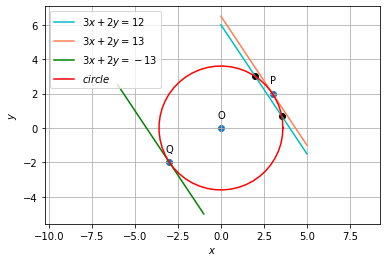
\includegraphics[width=1\columnwidth]{./solutions/4/2/2/figure.png}
\caption{Circle with tangent and intersection lines}
\label{eq:solutions/4/2/2/}
\end{figure}

